\documentclass[11pt,letterpaper]{article}
\usepackage[lmargin=1in,rmargin=1in,tmargin=1in,bmargin=1in]{geometry}
\usepackage{../style/homework}
\setbool{quotetype}{false} % True: Side; False: Under
\setbool{hideans}{false} % Student: True; Instructor: False

% -------------------
% Content
% -------------------
\begin{document}

\homework{12: Due 03/20}{Mitchell's mother has a problem\dots with me. Last Christmas, for example. She gave me a piece of exercise equipment and a lettuce dryer. So, to recap, I gave her a gorgeous pair of diamond earrings and she gave me a hint.}{Cameron Tucker, Modern Family}

% Problem 1
\problem{10} Find the equation of the line plotted below.
	\[
	\fbox{
	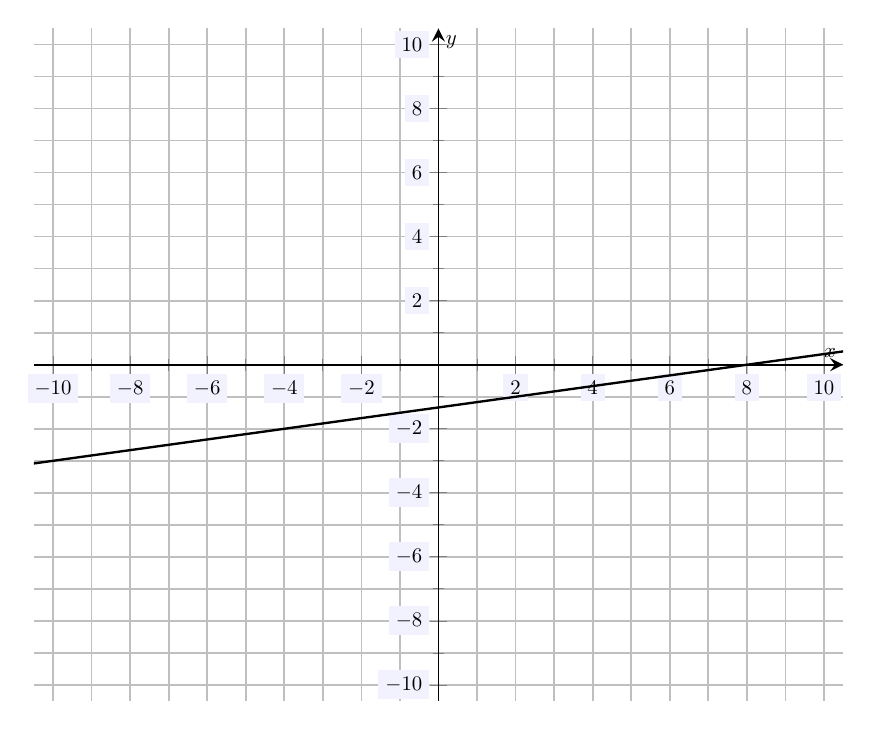
\begin{tikzpicture}[scale=1.5,every node/.style={scale=0.5}]
	\begin{axis}[
	grid=both,
	axis lines=middle,
	ticklabel style={fill=blue!5!white},
	xmin= -10.5, xmax=10.5,
	ymin= -10.5, ymax=10.5,
	xtick={-10,-8,-6,-4,-2,0,2,4,6,8,10},
	ytick={-10,-8,-6,-4,-2,0,2,4,6,8,10},
	minor tick = {-10,-9,...,10},
	xlabel=\(x\),ylabel=\(y\),
	]
	\addplot[line width= 0.02cm,samples=2,domain= -10.5:10.5] ({x},{-4/3 + 1/6*x});
	\end{axis}
	\end{tikzpicture}
	}
	\] \pspace

\sol Because the line is not vertical, we know that it must have the form $y= mx + b$ for some $m ,b$. We can see that the points $(-4, -2)$ and $(2, -1)$ lie exactly on the line. The slope of the line is then\dots
	\[
	m= \dfrac{\Delta y}{\Delta x}= \dfrac{-2 - (-1)}{-4 - 2}= \dfrac{-2 + 1}{-4 + -2}= \dfrac{-1}{-6}= \dfrac{1}{6}
	\]
But because the line contains the point $(2, -1)$, when $x= 2$ we know that $y= -1$. Therefore, \dots
	\[
	\begin{gathered}
	y= mx + b \\
	y= \dfrac{1}{6}\,x + b \\
	-1= \dfrac{1}{6} \cdot 2 + b \\
	-1= \dfrac{1}{3} + b \\
	b= -1 - \dfrac{1}{3} \\
	b= -\dfrac{4}{3}
	\end{gathered}
	\]
Therefore, the equation of the line is $y= \frac{1}{6}\,x - \frac{4}{3}= \frac{x - 8}{6}$. 



\newpage



% Problem 2
\problem{10} Find the equation of the following lines:
	\begin{enumerate}[(a)]
	\item The line through $(-1, 1)$ and $(6, -2)$.
	\item The line containing $(8, -1)$ with slope $\frac{4}{3}$.
	\item The line with $y$-intercept 5 and slope $-6$.
	\end{enumerate} \pspace

\sol 
\begin{enumerate}[(a)]
\item The slope of the line must be\dots
	\[
	m= \dfrac{\Delta y}{\Delta x}= \dfrac{1 - (-2)}{-1 - 6}= \dfrac{1 + 2}{-1 + (-6)}= \dfrac{3}{-7}= -\dfrac{3}{7}
	\] 
Then using the point-slope formula, $y= y_0 + m(x - x_0)$, the equation of the line is\dots
	\[
	y= 1 - \dfrac{3}{7} \big(x - (-1) \big)= 1 - \dfrac{3}{7} (x + 1)= 1 - \dfrac{3}{7}\, x - \dfrac{3}{7}= -\dfrac{3}{7}\,x + \dfrac{4}{7}= \dfrac{-3x + 4}{7}
	\] \pspace


\item Using the point-slope formula, $y= y_0 + m(x - x_0)$, the equation of the line is\dots
	\[
	y= -1 + \dfrac{4}{3} \left(x - 8 \right)= -1 + \dfrac{4}{3} \,x - \dfrac{32}{3}= \dfrac{4}{3}\, x - \dfrac{35}{3}= \dfrac{4x - 35}{3}
	\] \pspace

\item Using the slope-intercept form, $y= mx + b$, we have\dots
	\[
	y= -6x + 5
	\]
\end{enumerate}



\newpage



% Problem 3
\problem{10} Find the equation of the line with $x$-intercept $-4$ and $y$-intercept $6$. \pspace

\sol Because the line has $x$-intercept $-4$, it contains the point $(-4, 0)$. Because the line has $y$-intercept $6$, it contains the point $(0, 6)$. But then the slope of the line is\dots
	\[
	m= \dfrac{\Delta y}{\Delta x}= \dfrac{6 - 0}{0 - (-4)}= \dfrac{6 - 0}{0 + 4}= \dfrac{6}{4}= \dfrac{3}{2}
	\]
Then using the slope-intercept form of the line, $y= mx + b$, the line must be\dots
	\[
	y= \dfrac{3}{2}\,x + 6= \dfrac{3x + 12}{2}
	\]


\end{document}